\documentclass{beamer}

\mode<presentation>
{
  \usetheme{CambridgeUS}
  \usecolortheme{seagull}
  \setbeamercovered{transparent}
}

\usepackage[english]{babel}
\usepackage[latin1]{inputenc}
\usepackage{times}
\usepackage[T1]{fontenc} 
% Or whatever. Note that the encoding and the font should match. If T1
% does not look nice, try deleting the line with the fontenc.
\usepackage{amsmath}

\newcommand{\linespace}{\vskip 0.25cm}

\definecolor{MyForestGreen}{rgb}{0,0.7,0} 
\newcommand{\tableemph}[1]{{#1}}
\newcommand{\tablewin}[1]{\tableemph{#1}}
\newcommand{\tablemid}[1]{\tableemph{#1}}
\newcommand{\tablelose}[1]{\tableemph{#1}}

\definecolor{MyLightGray}{rgb}{0.6,0.6,0.6}
\newcommand{\tabletie}[1]{\color{MyLightGray} {#1}}

% The text in square brackets is the short version of your title and will be used in the
% header/footer depending on your theme.
\title[Concurrent Compaction in JVM GC]{Concurrent Compaction in JVM Garbage Collection}

% Sub-titles are optional - uncomment and edit the next line if you want one.
% \subtitle{Why does sub-tree crossover work?} 

% The text in square brackets is the short version of your name(s) and will be used in the
% header/footer depending on your theme.
\author[Jacob Opdahl]{Jacob P. Opdahl}


% The text in square brackets is the short version of your institution and will be used in the
% header/footer depending on your theme.
\institute[UMM]
{
  University of Minnesota, Morris \\[\baselineskip]
  \emph{opdah023@morris.umn.edu}
}

% The text in square brackets is the short version of the date if you need that.
\date[December 5, 2015] % (optional)
{December 5, 2015}

% Delete this, if you do not want the table of contents to pop up at
% the beginning of each subsection:
\AtBeginSection[]
{
  \begin{frame}<beamer>
    \frametitle{Outline}
    \tableofcontents[currentsection, hideothersubsections]
  \end{frame}
}

%\AtBeginSubsection[]
%{
%\begin{frame}<beamer>
%    \frametitle{Outline}
%    \tableofcontents[currentsection, currentsubsection]
%  \end{frame}
%}

\begin{document}

\begin{frame}
  \titlepage
\end{frame}

% For a 20-25 minute senior seminar talk you probably want something like:
% - Two or three major sections (other than the summary).
% - At *most* three subsections per section.
% - Talk about 30s to 2min per frame. So there should probably be between
%   15 and 30 frames, all told.



\section*{Overview}

\subsection*{Introduction}

\begin{frame}

\frametitle{Automatic Memory Management}

Implicit allocation and deallocation of memory

\linespace
\linespace

Languages: Java, C\#, Python, and more
\begin{itemize}
\item We focus on the Java Virtual Machine and languages it supports
\end{itemize}

\linespace
\linespace

Abstracts details away from the developer

\linespace

\begin{center}

\includegraphics[width=.3\textwidth]{Illustrations/garbage.jpg}
\end{center}

\end{frame}

\begin{frame}

\frametitle{Implicit Deallocation}

Memory is a finite resource

\linespace
\linespace

\emph{Garbage}: objects that are no longer reachable

\linespace
\linespace

\emph{Garbage Collection (GC)}: detecting and removing garbage

\linespace
\linespace
\linespace

\begin{center}

\includegraphics[width=.3\textwidth]{Illustrations/garbage.jpg}
\end{center}

\end{frame}

\begin{frame}

\begin{columns}
\begin{column}{0.65\textwidth}

\frametitle{Stopping the World}

GC requires processing resources

\linespace
\linespace

When only one processor is used, collectors \emph{stop the world}
% Need to get across that this can still be ueful.

\linespace
\linespace

Problem: applications today are subjected to increasing pauses
\begin{itemize}
\item More memory
\item More strenuous applications
\end{itemize}

\linespace
\linespace

Use parallel processing to solve!
\end{column}
\begin{column}{0.35\textwidth}

\begin{center}

\includegraphics[width=.8\textwidth]{Illustrations/meme.jpg}
\end{center}

\end{column}
\end{columns}

\end{frame}



\subsection*{Outline}

\begin{frame}
  \frametitle{Outline}
  \tableofcontents  
  %\tableofcontents[hidesubsections]
\end{frame}



\section[Background]{Background}

\subsection[GC Basics]{Garbage Collection}

\begin{frame}

\frametitle{Memory}

% Mention this is the shared memory for the JVM process and all its tasks.
\emph{Heap}: contiguous memory location used by the JVM
\begin{itemize}
\item Objects are stored here
\end{itemize}

\linespace
\linespace

% Mention it has more purposes, but for our sake, it's a way to access the heap.
\emph{Stack}: memory for short-lived, method-specific values
\begin{itemize}
\item Stores \emph{references}: memory addresses of objects
\end{itemize}

\linespace
\linespace

\begin{center}
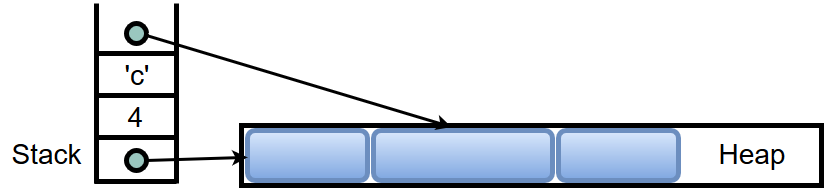
\includegraphics[width=.8\textwidth]{Illustrations/stack_and_heap.png}
\end{center}

\end{frame}

\begin{frame}

\frametitle{GC Cycle}

\emph{Set Condemnation}: determine which objects are garbage 

\linespace
\linespace

\emph{Compaction}: reclaim memory while fighting heap fragmentation

\linespace
\linespace
\linespace

% Don't mention root-level, global objects. Just say objects reached by chaining references from main.
Set condemnation done by \emph{tracing}
\begin{itemize}
\item Detect all reachable objects by chaining references
\end{itemize}

\end{frame}

\begin{frame}

\frametitle{Compaction}

% Need to mention here how to-space and from-space can actually have some areas of memory in common. They are not always distinct places.

Consists of two steps
\begin{itemize}
\item \emph{Relocation}: move objects 
\begin{itemize}
\item \emph{from-space} and \emph{to-space}
\end{itemize}
\item \emph{Remapping}: update object references
\end{itemize}

\linespace

%Make sure to point out that this is the heap.
\begin{center}
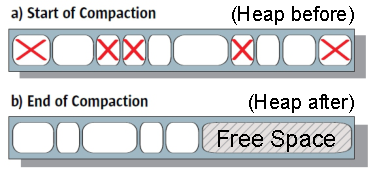
\includegraphics[width=.60\textwidth]{Illustrations/bg_compaction.pdf}
\end{center}

% The compaction process will be our focus, but we want it done concurrently. In order to know what that means though, we need to understand a bit about parallel processing.

\end{frame}



\subsection[PP Basics]{Parallel Processing}

\begin{frame}

\frametitle{Processes and Threads}

\begin{columns}
\begin{column}{0.7\textwidth}

% Mention two word processors being open means two processes.
\emph{Process}: instance of a program being run
\begin{itemize}
\item Examples: JVM, word processor
\item Has its own memory space
\end{itemize}

\linespace
\linespace

\emph{Thread}: sequence of independent instructions that can run on its own
\begin{itemize}
\item Component of a process %MENTION HERE THAT THREADS SHARE THE HEAP (Or the memory the process has). That's why the JVM has Stacks, so threads can do their own work.
\item Possible to run multiple in parallel
\end{itemize}

\linespace
\linespace

\emph{Parallel Processing}: running multiple threads simultaneously with multiple processors

\end{column}

\begin{column}{0.30\textwidth}

\begin{center}
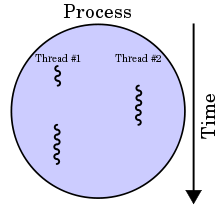
\includegraphics[width=1.0\textwidth]{Illustrations/multithreading.png} \\
{\small \url{wikipedia.org/wiki/Thread_\%28computing\%29}}
\end{center}

\end{column}
\end{columns}

\end{frame}

\begin{frame}

\frametitle{Synchronization}

\only<1>{

\begin{columns}
\begin{column}{0.60\textwidth}
Threads do not coordinate automatically \\
\begin{itemize}
\item Independent instructions!
\end{itemize}

\linespace
\linespace

Poses new challenges
\begin{itemize}
\item Example: losing object modifications
\end{itemize}

\linespace
\linespace

Need to keep threads synchronized
\end{column}

\begin{column}{0.4\textwidth}

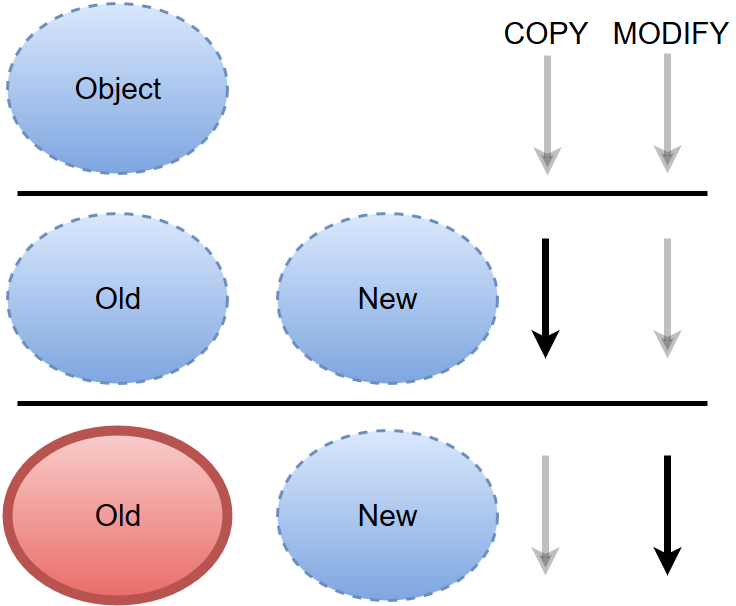
\includegraphics[width=1.0\textwidth]{Illustrations/sync_issue_example.png}

\end{column}
\end{columns}

}

\only<2>{

% DO NOT do the traffic example. Wastes time.
\emph{Read Barrier}: instructions to run before a thread accesses memory

\linespace
\linespace
\linespace

\begin{center}
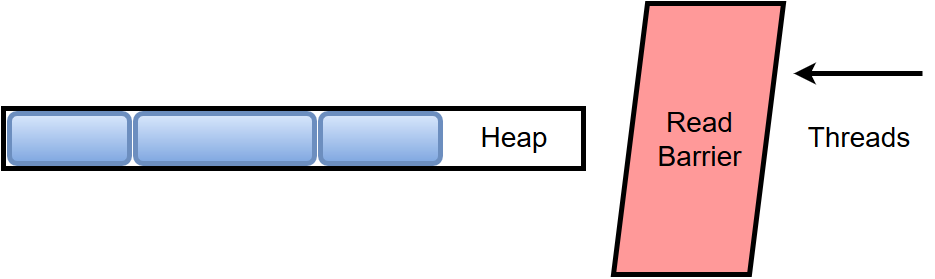
\includegraphics[width=.70\textwidth]{Illustrations/read_barrier.png}
\end{center}

}

\end{frame}



\subsection[GC with PP]{Garbage Collection with Parallel Processing}

\begin{frame}

\frametitle{Concurrency}

We distinguish between application threads and GC threads

\linespace
\linespace

\emph{Concurrent GC}: collector runs at the same time as the application
\begin{itemize}
\item Does not stop the world
\end{itemize}

\linespace
\linespace

Our focus: concurrent compaction!

\end{frame}



\section[C4]{Continuously Concurrent Compacting Collector (C4)}

\begin{frame}

\frametitle{Continuously Concurrent Compacting Collector (C4)}

Researchers: G.~Tene, B.~Iyengar, and M.~Wolf at Azul Systems

\linespace
\linespace
\linespace
\linespace

\begin{center}
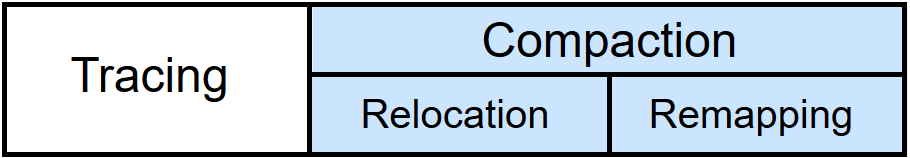
\includegraphics[width=.85\textwidth]{Illustrations/gc_cycle_locator_compaction.png}
\end{center}

\end{frame}



\subsection*{Explanation}

\begin{frame}

\frametitle{Loaded Value Barrier (LVB)}

%Mention that this is during compaction!
% REFRESHER ON FROM AND TO SPACE HERE!!!
Read barrier protects from-space from application threads
\begin{itemize}
\item From-space: where objects were located before moving
\end{itemize}

\linespace
\linespace

Rule: application can only use moved objects
\begin{itemize}
\item If a thread breaks this, the barrier will correct the situation
\end{itemize}

\linespace
\linespace

This facilitates concurrent relocation and remapping

\end{frame}

\begin{frame}

\frametitle{Concurrent Relocation}

\only<1>{

GC threads simply relocate objects

\linespace
\linespace

All references point to from-space!
\begin{itemize}
\item Application threads certain to trigger LVB
\end{itemize}

\linespace

\begin{center}
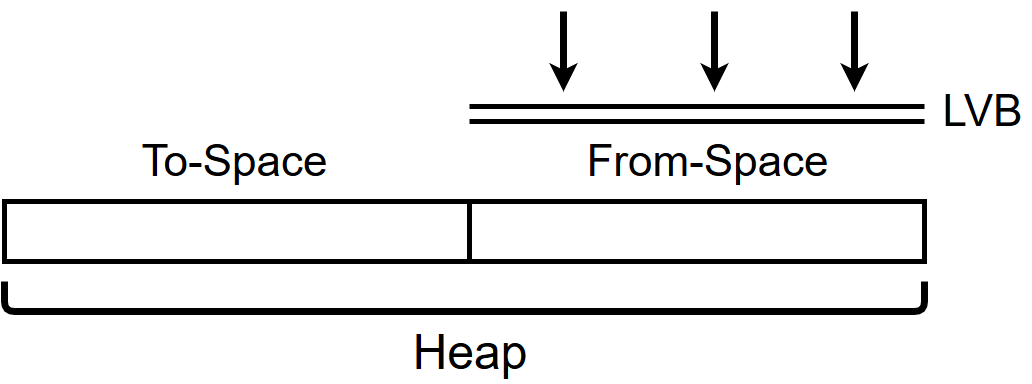
\includegraphics[width=.80\textwidth]{Illustrations/c4_lvb_relocation.png}
\end{center}

}

\only<2>{

LVB instructions for applications threads
\begin{itemize}
\item If the object was moved, find it
\item If the object is being moved, wait
\item If the object is unmoved, move it
\end{itemize}

\linespace
\linespace

In all cases, update the reference after using the object in to-space

}

\end{frame}

\begin{frame}

\frametitle{Concurrent Remapping}

To update all references, need to traverse all reachable ones

\linespace
\linespace

Combine remapping with next tracing phase

\begin{center}
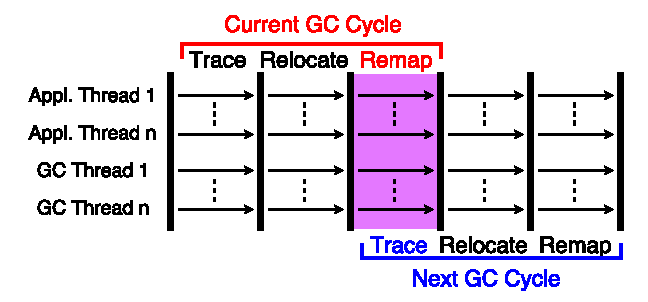
\includegraphics[width=.8\textwidth]{Illustrations/c4Mapping_rough_figure_5.pdf}
\end{center}

\end{frame}



\subsection*{Test Results}

\begin{frame}

\frametitle{Testing Environment}

Tested against two collectors with non-concurrent compaction

\linespace
\linespace

Improvements from concurrent compaction

\linespace
\linespace

Server environments used

\end{frame}

\begin{frame}

\frametitle{Results}

\begin{columns}
\begin{column}{0.5\textwidth}

%When explaining the test results, explain the intended environment is large server software.

\color[RGB]{135,35,142}C4\color{black}:
\begin{itemize}
\item Fastest response times
\item Maintains them for largest range of heap sizes
\item Least impact on application
\end{itemize}

\end{column}

%Really emphasive and say that higher values means faster response times.
\begin{column}{0.5\textwidth}
\begin{center}
Worst Case Response Times
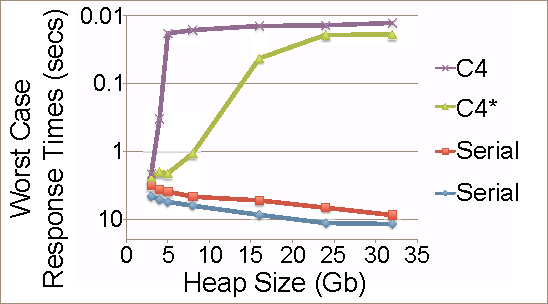
\includegraphics[width=.89\textwidth]{Illustrations/c4_results.pdf}
\end{center}
\end{column}
\end{columns}

\end{frame}



\section[FPP]{Field Pinning Protocol}

\begin{frame}

\frametitle{Field Pinning Protocol (FPP)}

Implemented into a \emph{host} GC algorithm

\linespace
\linespace

%Mention that it also differs in that since it is designed for a host gc algorithm,
%it is designed with less-specialized jvm environments in mind (not just server)
Differs from C4 - barrier-free!

\linespace
\linespace

Researchers: E.~\"{O}sterlund and W.~L\"{o}we at Linnaeus University

\linespace
\linespace
\linespace

\begin{center}
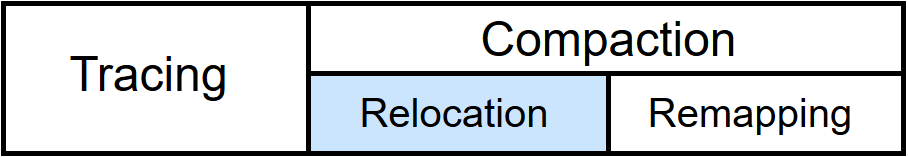
\includegraphics[width=.85\textwidth]{Illustrations/gc_cycle_locator_relocation.png}
\end{center}

\end{frame}



\subsection*{Explanation}

\begin{frame}

\frametitle{Hazard Pointers}

\emph{Hazard Pointers}: values that show which objects an application thread is accessing

\linespace
\linespace

Inform other threads of objects that are in use

\linespace
\linespace

Main goal: safely access objects without worrying about relocation

\end{frame}


\begin{frame}

\frametitle{Example}

\begin{columns}
\begin{column}{0.45\textwidth}
	\begin{itemize}
	\item Object = Coffee 
	\item \color{red}{Application Thread = Person w/ Coffee Cup} 
	\only<2->{\item \color{blue}{Relocation Thread = Person}}
	\only<2->{\item \color{black}{* = Responsible}} 
	\only<2->{\item ! = Impeded}
	\end{itemize}
\end{column}
\begin{column}{0.55\textwidth}
	\only<1>{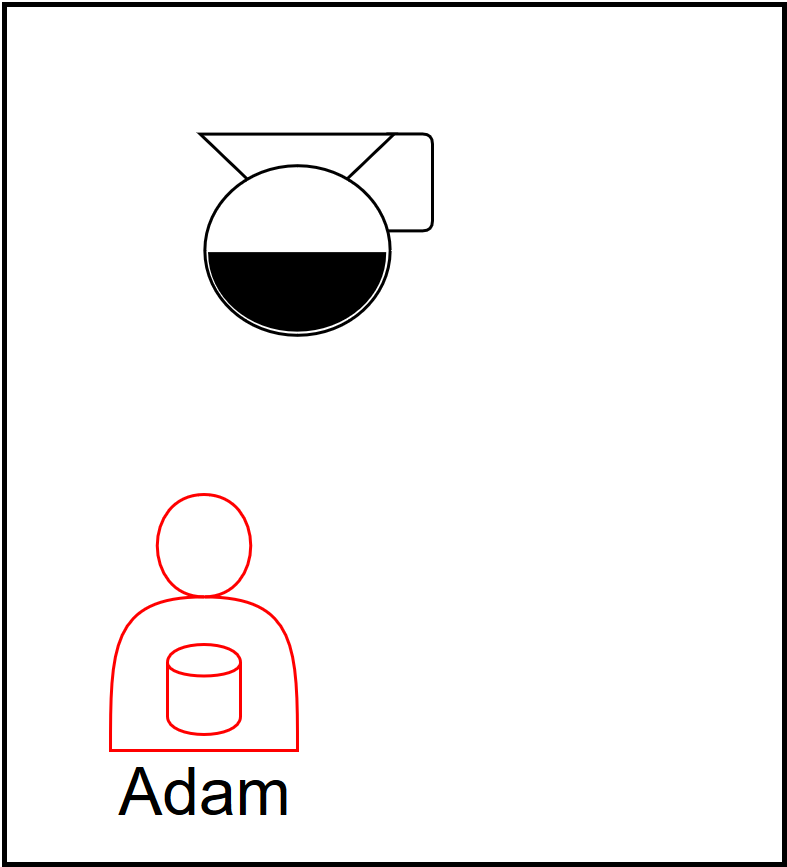
\includegraphics[width=.95\textwidth]{Illustrations/coffeeLineNew1.png}}
	\only<2>{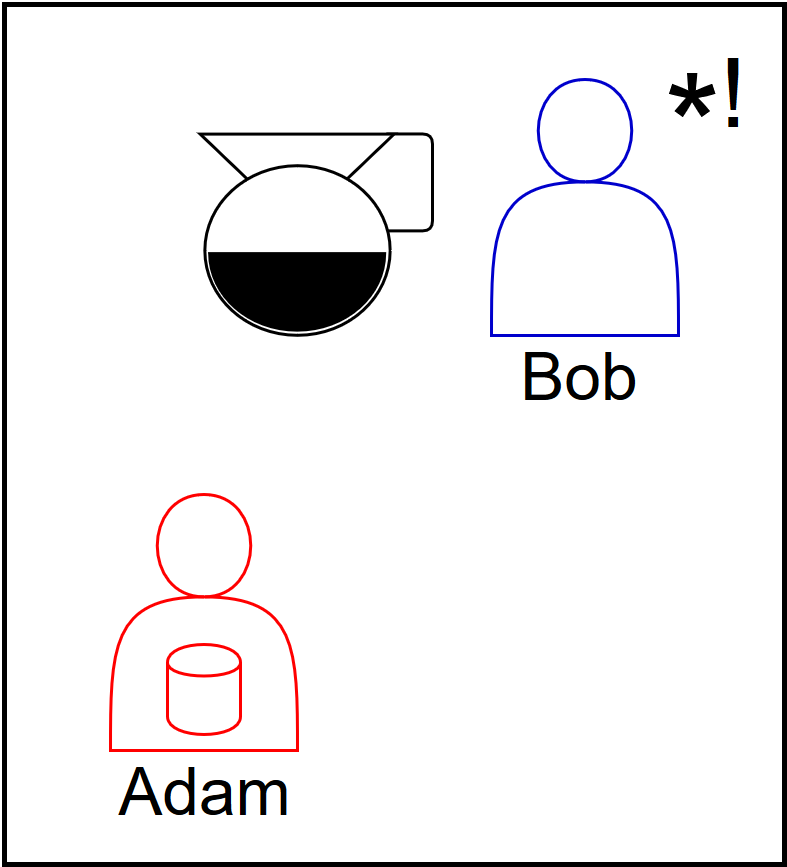
\includegraphics[width=.95\textwidth]{Illustrations/coffeeLineNew2.png}}
	\only<3>{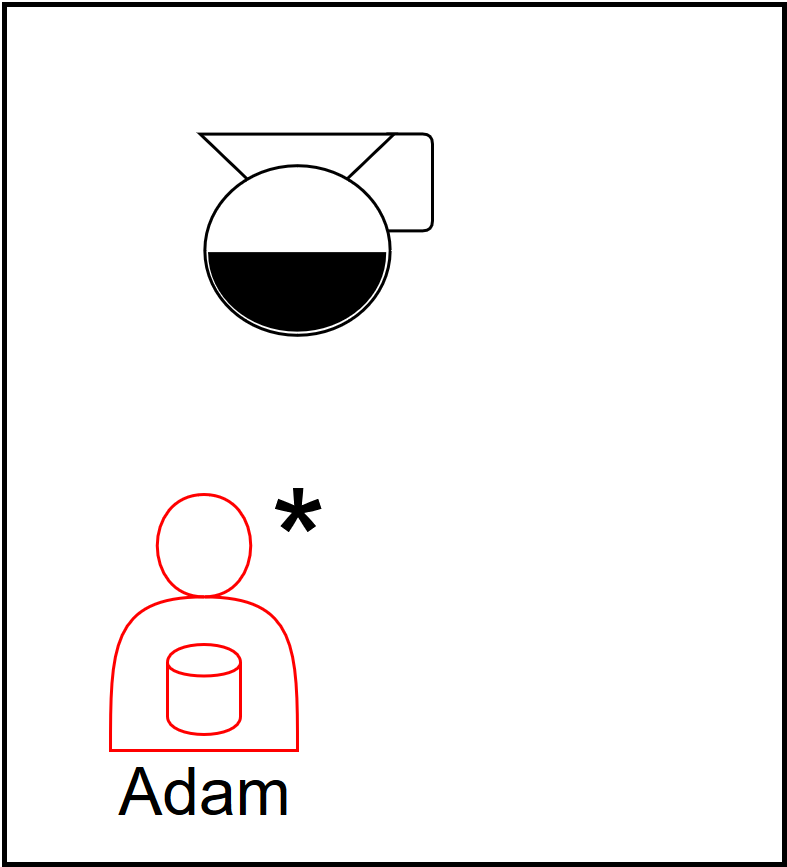
\includegraphics[width=.95\textwidth]{Illustrations/coffeeLineNew3.png}}
	\only<4>{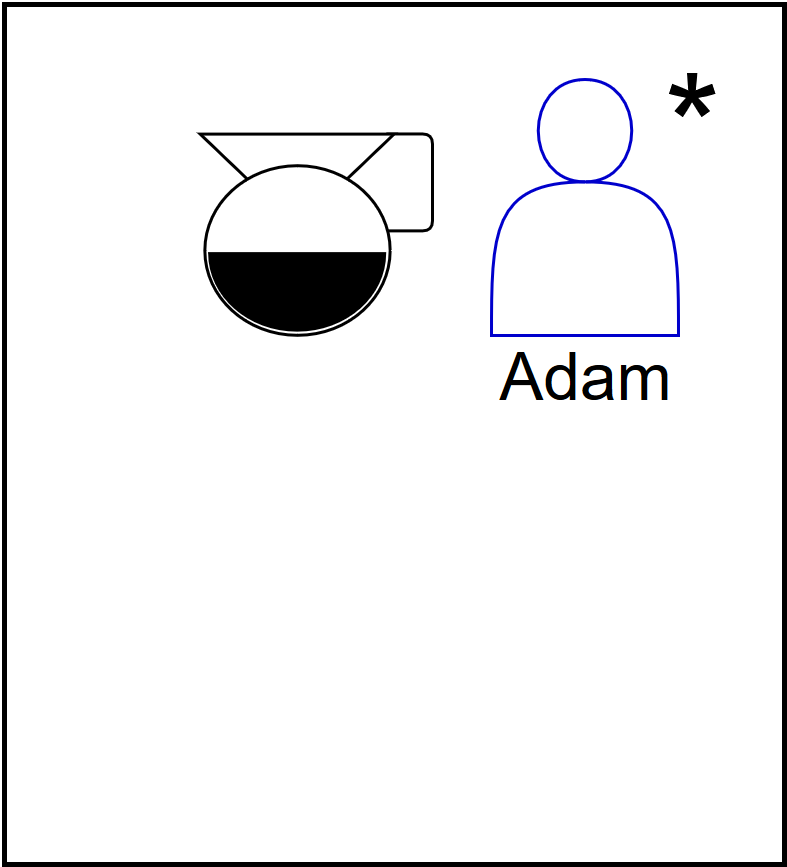
\includegraphics[width=.95\textwidth]{Illustrations/coffeeLineNew4.png}}
	\only<5>{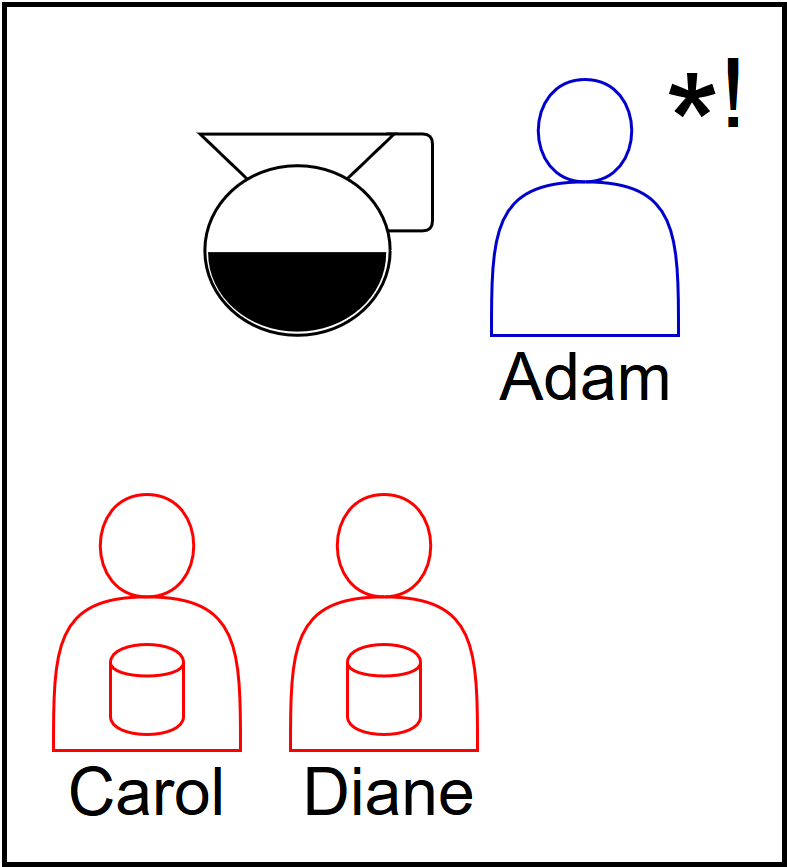
\includegraphics[width=.95\textwidth]{Illustrations/coffeeLineNew5.png}}
	\only<6>{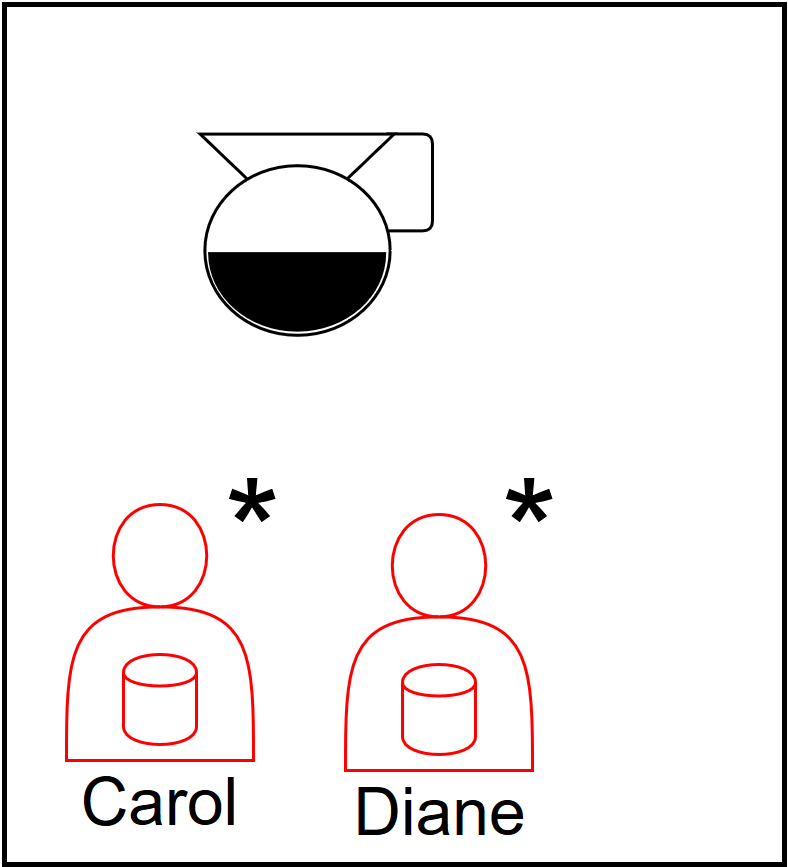
\includegraphics[width=.95\textwidth]{Illustrations/coffeeLineNew6.png}}
	%If anyone asks how this is bounded, it's because threads consume their blame atomically,
	%so a thread gets rid of all its blame at once.
\end{column}
\end{columns}

\end{frame}


\begin{frame}

\frametitle{Concurrent Relocation and Responsibility}

%If time allows and feedback demands, could break this into multiple slides to not have so much text
%on one as well as to refer back to the example and characters more.

\emph{Responsibility}: thread required to try relocating an object
\begin{itemize}
\item Comes from hazard pointers (coffee cups) impeding copying
\end{itemize}

\linespace
\linespace

Relocation with FPP
\begin{itemize}
\item GC threads attempt to relocate objects
\item Impeding application threads are made responsible
\begin{itemize}
\item When finished with the object, try to move
\end{itemize}
\item Responsibility passed to impeding threads until relocation succeeds
\end{itemize}
% Say here that paper specifies ways of ensuring this doesn't go on forever, but not enough time to discuss.

\end{frame}



\subsection*{Test Results}

\begin{frame}

\frametitle{Testing Environment}

Implemented in the Garbage-First (G1) Garbage Collector
\begin{itemize}
\item Concurrent tracing and remapping
\item Relocation requires stop-the-world pauses
\end{itemize}

\linespace
\linespace

Tested against the default G1 collector

\linespace
\linespace

Improvements from solely concurrent relocation

\end{frame}

\begin{frame}

\frametitle{Results}

\begin{columns}
\begin{column}{0.5\textwidth}

\color{red}G1 with FPP \color{black}on average 50\% shorter delays than \color{blue}standard G1\color{black}
\begin{itemize}
\item Less impact on application performance
\end{itemize}

\linespace
\linespace

Concurrent relocation without barriers is feasible!

\end{column}

\begin{column}{0.5\textwidth}

% EXPLAIN WHAT IS ON THIS TABLE BETTER. DON'T TALK ABOUT STUFF THAT ISN'T ON HERE UNLESS IT'S NEEDED.
\begin{center}
Average GC Delays
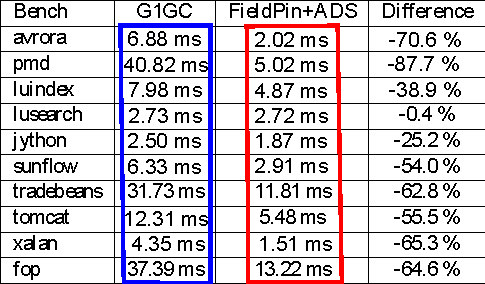
\includegraphics[width=.90\textwidth]{Illustrations/fpp_results_3.pdf}
\end{center}
\end{column}
\end{columns}

\end{frame}



\section[Conclusions]{Conclusions}

\begin{frame}

\frametitle{Conclusions}

Moving toward concurrent compaction without barriers
\begin{itemize}
\item C4 - heavily relies on barriers
\item FPP - barrier-free
\end{itemize}

%\linespace
%\linespace
%
%Different approaches to prioritizing GC vs application
%\begin{itemize}
%\item C4 - focus on GC
%\item FPP - focus on application
%\end{itemize}

\linespace
\linespace

Tough to compare them directly

\linespace
\linespace

All tests showed that concurrency can improve application performance
\begin{itemize}
% MENTION C4 is server-targeting and FPP is more general.
\item Approach used will depend on intended environment
\end{itemize}

\end{frame}

\begin{frame}
	\frametitle{Thanks for your time!}
	
	\begin{center}
	{\huge Questions?}
	\end{center}	
	
	\linespace
	\linespace	
	
	\begin{center}
	Contact: opdah023@morris.umn.edu
	\end{center}
	
\end{frame}



\section*{References}

\begin{frame} 
	\frametitle{References} 

\begin{thebibliography}{lskdjf}

\bibitem{Tene:2011}
G.~Tene, B.~Iyengar, and M.~Wolf.
\newblock C4: the continuously concurrent compacting collector.
\newblock 2011 ACM SIGPLAN International Symposium on Memory Management (ISMM 2011). ACM, New York, NY, USA, 79-88.

\bibitem{Lowe:2015}
E.~\"{O}sterlund and W.~L\"{o}we.
\newblock Concurrent compaction using a field pinning protocol. 
\newblock 2015 ACM SIGPLAN International Symposium on Memory Management (ISMM 2015). ACM, New York, NY, USA, 56-69.

\linespace
\linespace
\linespace
\begin{center}
\color{black}See the UMM Opdahl Fall '15 paper for additional references.
\end{center}


\end{thebibliography}

\end{frame} 



\end{document}


